\section{Non-Collateralized Bond}
\label{app:non-collat-bond}
At the time of writing, there are more than a thousand implemented blockchains working. One of our concerns about the non-collateralized bond component is the possibility of using CHECKSEQVERIFY. If the blockchain of interest does not support this type of opcode we can not use this type of bond. For fixing this problem we design ABCD which does not need to use this opcode. Fig.~\ref{fig:non-collat-bond-no-checkseq} well demonstrates the mechanism of this bond by adding a new stage named {\it delay keeper}.


The diagram of this bond is shown in Fig~\ref{fig:non-collat-bond} 
\begin{figure}
    \centering
    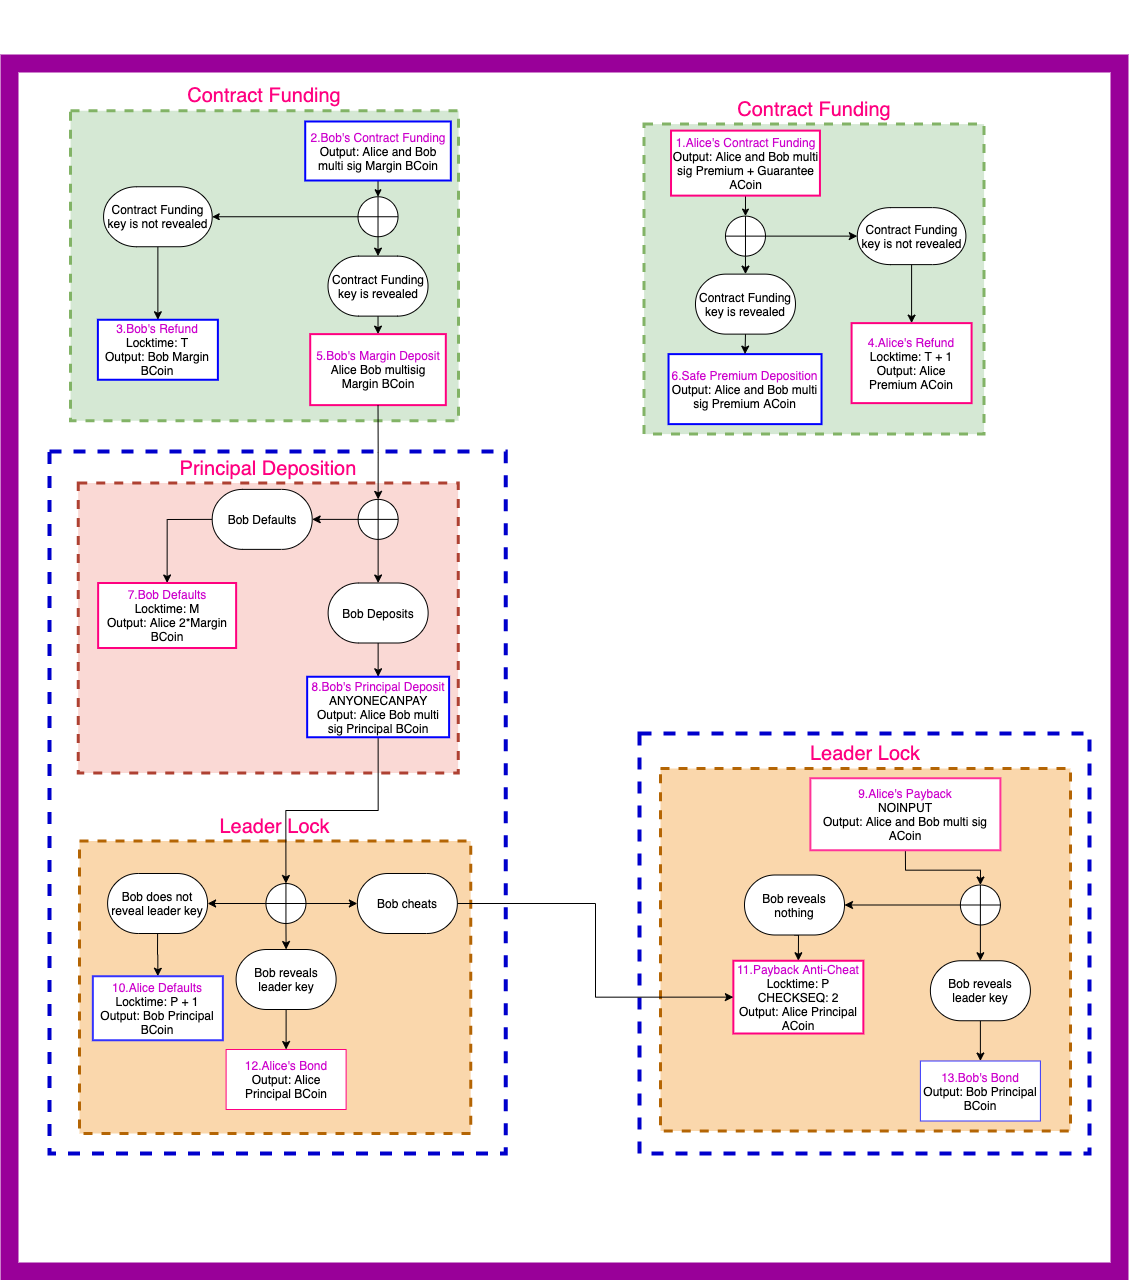
\includegraphics[width=\textwidth]{figures/non-collateralized-bond-checkseq.png}
    \caption{Non-collateralized bond}
    \label{fig:non-collat-bond}
\end{figure}

\begin{figure}
    \centering
    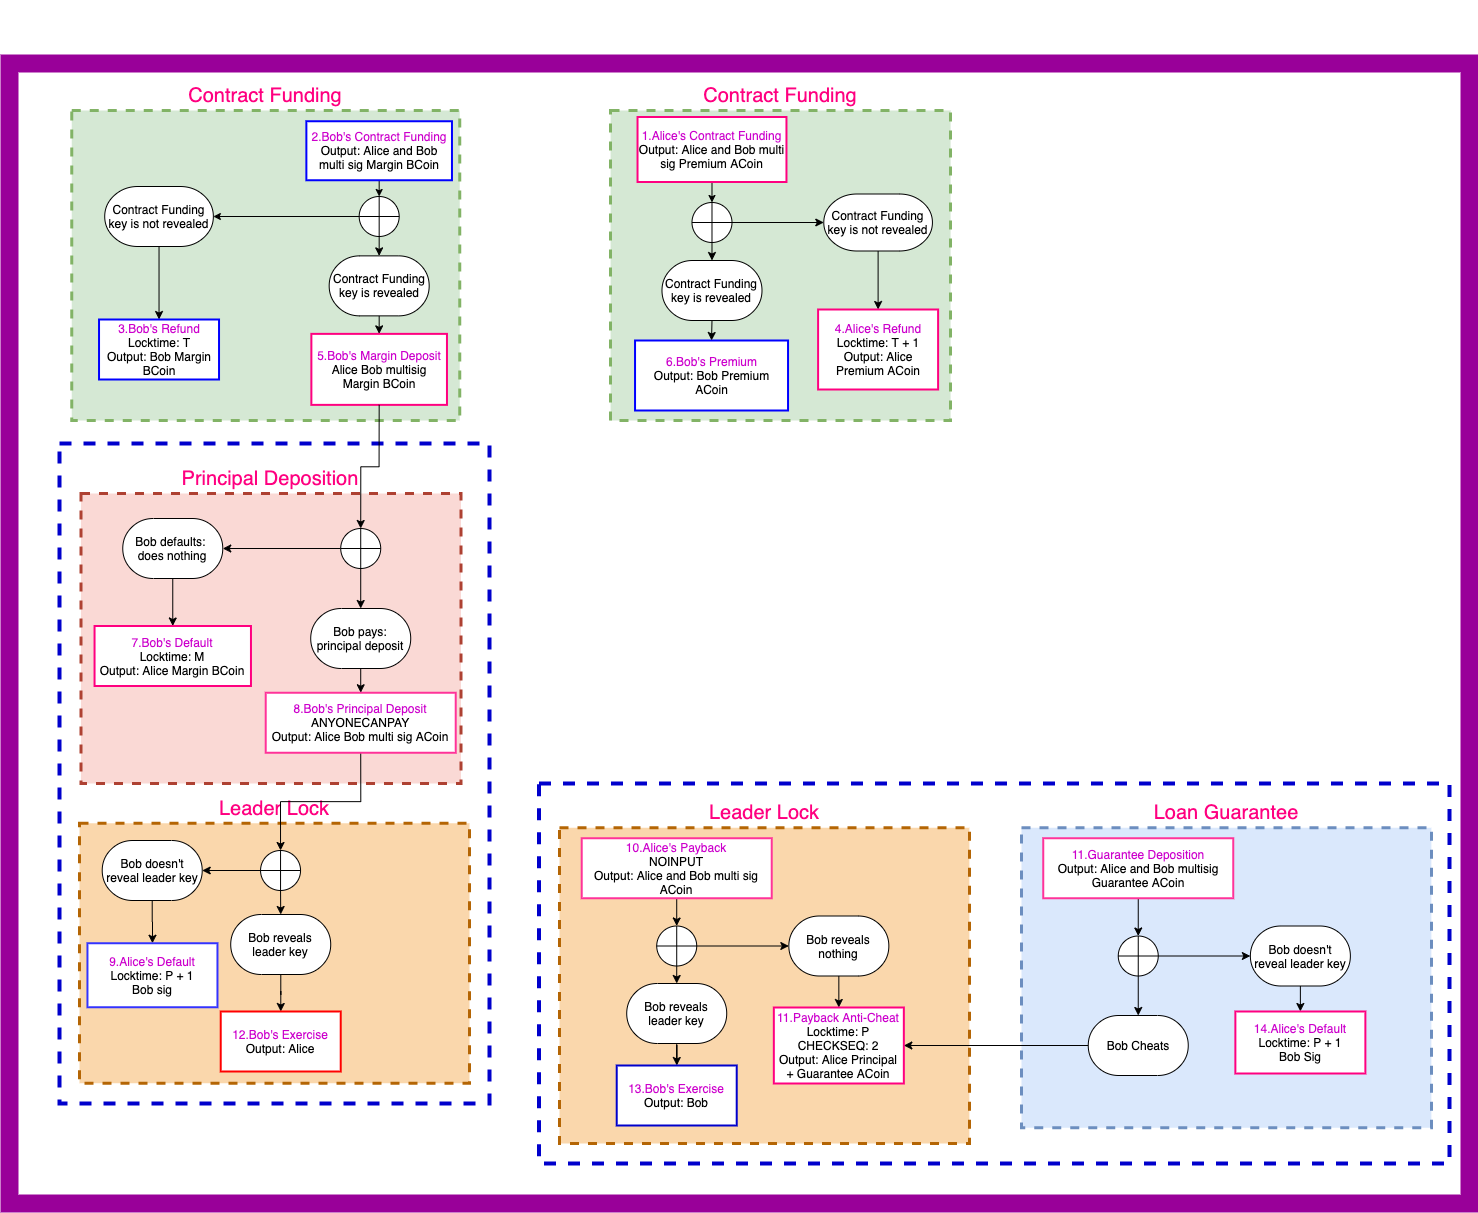
\includegraphics[width=\textwidth]{figures/non-collateralized-bond-checkseq-cross-chain.png}
    \caption{Crosschain Non-collateralized bond}
    \label{fig:cross-chain-non-collat-bond}
\end{figure}


\begin{itemize}
    \item \textbf{Bond Funding}: Same as previous type except for the Alice premium the 546 extra Satoshis is no longer needed.
    
    \item \textbf{Principal Deposition}: We give Bob the option for depositing a lesser amount of money than his principal as margin. Bob has M locktime to deposit the extra money to fulfill his principal. If Bob defaults on his margin, Alice will take the ownership of his margin by broadcasting the default transaction.
    
    \item \textbf{Leader Key}: If the principal deposition stage ends well and Bob deposits his principal before the locktime, Alice has P - 2 locktime to use her bond to payback Bob's money. Obviously the payback transaction is NOINPUT since no body knows its input transactions in the first place. The desired procedure of this stage is: 1) Alice succeeds to payback Bob's bond and Bob reveals the \keyone key. 2) Alice fails to broadcast the payback transaction, so that Bob avoids exposing the \keyone key and his principal is sent back to himself. For satisfying the second goal, Bob gives Alice P + 1 locktime to convince him to reveal the \keyone key and if her time is up, he will broadcast the Alice-defaults transaction on chain which revert the bond process. For the first goal, there is a transaction which sends the payback transaction to Bob by revealing the \keyone key. Though Bob can avoid revealing the \keyone key even if Alice fulfills her payback transaction. If Bob tries to cheat on Alice by doing this, Alice can send the anti-cheat transaction on chain which sends her principal and an amount of punishment from Bob's bond to herself. We reach all the desired goals, however, if we do not use CHECKSEQVERIFY for spending the payback transaction on the anti-cheat transaction, Alice can wait until P locktime and eventually in the very last moment deposit her principal and cheat on Bob. For fixing this issue, The output of the payback transaction is marked as CHECKSEQVERIFY 2 which prevents Alice from sending anti-cheat transaction before 2 relative locktime after her payback transaction.
     
\end{itemize}


By using the above form, we can not offer decentralized non-collateralized bond to parties that are in different blockchains, because the anti-cheat transaction has inputs from both Alice's and Bob's sides. For overcoming this issue, before settling any bond contract, Bob which is considered to be an exchange or somebody who has reasonable amount of money in different chains, can deposit some money in every desired chain as a bond guarantee equal to the punishment amount. In this way, Bob can offer his customers a cross-chain bond service which accepts his payback money in the other chain. This modification can be seen in Fig.\ref{fig:cross-chain-non-collat-bond}


